\documentclass[9pt]{beamer}
\usepackage{silence}
\WarningFilter{beamerthememetropolis}{You need to compile with XeLaTeX or LuaLaTeX to use the Fira fonts}
\usetheme[titleformat = smallcaps, block = fill, progressbar = frametitle]{metropolis}
\title{\Huge Elements of Mathematics}
%---------------------------------%
% PACKAGES
%---------------------------------%
% Input encoding.
\usepackage[utf8]{inputenc} % For accents in spanish: transforms "á" into "\'a"
\usepackage[T1]{fontenc} % Output encoding. Use to avoid silly problems on the output.
                         % See: http://tex.stackexchange.com/questions/664/why-should-i-use-usepackaget1fontenc
\usepackage[sfdefault]{FiraSans}
\usepackage{FiraMono}
% AMS packages
\usepackage{amsmath}
\usepackage{amsfonts}
\usepackage{amssymb}
\usepackage{amsthm}
% Matrices
\usepackage{mathtools}
\newcommand{\verteq}{\rotatebox{90}{$\,=$}}
\usepackage{gauss}
% Customization for augmented matrices; 
% see https://tex.stackexchange.com/questions/146723/how-to-typeset-row-operations-on-augmented-matrix
% Patch gauss macros for doing their work in `align'
% and other amsmath environments; see http://tex.stackexchange.com/questions/146532/
\usepackage{etoolbox}
\makeatletter
\patchcmd\g@matrix
    {\vbox\bgroup}
    {\vbox\bgroup\normalbaselines} % restore the standard baselineskip
    {}{}
\makeatother
\newcommand{\BAR}{%
    \hspace{-\arraycolsep}%
    \strut\vrule % the `\vrule` is as high and deep as a strut
    \hspace{-\arraycolsep}%
}
% Math blackboard font
\usepackage{bbm}
% Fonts
\usepackage{lmodern} 
% \usepackage[sfdefault]{FiraSans}
\usepackage[normalem]{ulem}
\usepackage{eulervm}
% Graphics
\usepackage{graphicx} 
\usepackage{float}
\usepackage{subcaption}
\usepackage{wrapfig}
\usepackage{animate}
\usepackage{caption}
% Algorithms
\usepackage[ruled]{algorithm2e}
\newcommand{\lIfElse}[3]{\lIf{#1}{#2 \textbf{else}~#3}}
% Boxes
\usepackage[most]{tcolorbox}
% For reference enumerations lists
\usepackage{enumitem}
% \setlist{labelwidth = \widthof{0.}, leftmargin = {\labelwidth+\labelsep}, 
%         rightmargin = \leftmargin} % Setting left marging = right marging in itemize envirnment
% Import icons
\usepackage{fontawesome}
% Hyperlink
\usepackage{hyperref}
\hypersetup{
	final,
    bookmarksnumbered=true,
    bookmarksopen=true,
    bookmarksopenlevel=0,
    unicode=false,          % non-Latin characters in Acrobat?s bookmarks
    pdftoolbar=true,        % show Acrobat?s toolbar?
    pdfmenubar=true,        % show Acrobat?s menu?
    pdffitwindow=false,     % window fit to page when opened
    pdftitle={Introduction to Mathematics},    % title
    pdfdisplaydoctitle=true, %display document title instead of file name in title bar
    pdftoolbar=true,
    pdfmenubar=true,
    pdflang={English},
    pdfauthor={Abel Guada Azze},     % author
    pdfsubject={Introduction to Mathematics},   % subject of the document
    pdfcreator={Abel Guada Azze},   % creator of the document
    pdfproducer={Abel Guada Azze}, % producer of the document
    pdfkeywords={Mathematics} {introduction}, % list of keywords
    pdfnewwindow=true,      % links in new window
    breaklinks=true,
    hidelinks,
    colorlinks,
    linkcolor=black,          % color of internal links (change box color with linkbordercolor)
    citecolor=black,        % color of links to bibliography
    filecolor=cyan,      % color of file links
    urlcolor=magenta           % color of external links
}
%----------------------------------- Tikz
\usepackage{tikz}
\usepackage{pgfplots}
% \pgfplotsset{compat=1.18}
% \usepackage{tkz-euclide}
\usetikzlibrary{shapes,arrows.meta,matrix,positioning,calc}
\newcommand{\tikzmark}[1]{\tikz[baseline,remember picture] \coordinate (#1) {};}
% ---------- Helpers: 2-set and 3-set Venns ----------
% \VennTwoCounts{LabelA}{LabelB}{onlyA}{both}{onlyB}{Neither}{Universe}
\newcommand{\VennTwoCounts}[7]{%
  \begin{tikzpicture}[scale=1.0,baseline=(current bounding box.center)]
    \def\r{1.8}   % circle radius (cm)
    \def\dx{2.35} % distance between centres (cm)
    \def\pad{0.60} % padding between circles and rectangle (cm)

    \coordinate (A) at (0,0);
    \coordinate (B) at (\dx,0);

    % Universe rectangle (outline only)
    \draw[line width=.8pt, rounded corners=2pt]
      ($(A)+(-\r-\pad,-\r-\pad)$) rectangle ($(B)+(\r+\pad,\r+\pad)$);

    % Set fills + outlines
    \fill[black!8] (A) circle (\r);
    \fill[black!8] (B) circle (\r);
    \draw[line width=.8pt] (A) circle (\r);
    \draw[line width=.8pt] (B) circle (\r);

    % Universe label (top-left inside the box)
    \node[font=\scriptsize,anchor=north west]
      at ($(A)+(-\r-\pad+0.12,\r+\pad-0.12)$) {#7};

    % Set labels
    \node[font=\small\bfseries] at ($(A)+(0,0.68*\r)$) {#1};
    \node[font=\small\bfseries] at ($(B)+(0,0.68*\r)$) {#2};

    % Counts
    \node[font=\small] at ($ (A)+(-0.60*\r,-0.05*\r) $) {#3}; % only A
    \node[font=\small] at ($ .5*(A)+.5*(B) $) {#4};           % both
    \node[font=\small] at ($ (B)+(0.60*\r,-0.05*\r) $) {#5};  % only B
    \node[font=\small]
      at ($ (B)+(\r+0.3*\pad,0.78*\r) $) {#6};                % outside
  \end{tikzpicture}%
}


%---------------------------------%
% Biblio
%---------------------------------%

%---------------------------------%
% SETTINGS
%---------------------------------%
% displays sections and subsections numbered in the TOC
\setbeamertemplate{section in toc}[sections numbered]
% \setbeamertemplate{subsection in toc}[subsections numbered]
% gets rid of bottom navigation bars
\setbeamertemplate{footline}{}
% gets rid of bottom navigation symbols
\setbeamertemplate{navigation symbols}{}
% sets images' path
\graphicspath{{img/}}
% resets footnote counter at the beginning of each section
\AtBeginEnvironment{frame}{\setcounter{footnote}{0}}
% beamer margins
\setbeamersize
{
    text margin left=3mm,
    text margin right=3mm,
    % sidebar width left=.0cm,
    % sidebar width right=.0cm,
    % description width,
    % description width of=,
    % mini frame size=,
    % mini frame offset
}
% redefines block environment to add small space between title and content
\let\oldblock\block
\let\endoldblock\endblock
\renewenvironment{block}[1]
    {\begin{oldblock}{#1}
        \vspace{0.1cm}
    }
    { 
    \end{oldblock}
    }

%---------------------------------%
% SETTINGS
%---------------------------------%
%---------------------------------%
% TITLE PAGE
%---------------------------------%
\setbeamertemplate{title page}{
    \vspace{-0.4cm}
    
    \textcolor{CUNEForange}{\rule{\textwidth}{0.05cm}}
    \vspace{-0.65cm}
    
    \begin{minipage}{0.2\textwidth}
        \includegraphics[width = 2.0cm]{Logo-CUNEF.png}
    \end{minipage}
    \begin{minipage}{0.7\textwidth}
        
        \quad \Huge \usebeamertemplate*{title}
        
    \end{minipage}    
    \vspace{-0.25cm}
    
    \textcolor{CUNEForange}{\rule{\textwidth}{0.05cm}}
    \vspace{1.5cm}

    \begin{minipage}{0.075\textwidth}
        
    \end{minipage}\hfill\textcolor{CUNEForange}{\vrule\vrule\vrule}
    \begin{minipage}{0.825\textwidth}
        \begin{itemize}[leftmargin = *, label= $ $]
            \item {\hspace{1.05pt} \faUser\quad Abel Guada Azze}
            \item {\hspace{0pt} \faEnvelope\quad \href{mailto:abel.guada@cunef.edu}{abel.guada@cunef.edu}}
            \item {\hspace{0pt} \faSuitcase\quad F4.5 - C. de Leonardo Prieto Castro, 2}
            \item {\hspace{0pt} \faUniversity\ \ \ Department of Quantitative Methods - CUNEF Universidad}
            \item {\hspace{0pt} \faGraduationCap\ \ \ Bachelor in Philosophy, Politics and Economics}
        \end{itemize}
    \end{minipage}
}
\setbeamertemplate{title}{
  \linespread{1.0}%
  \inserttitle%
  \par%
  \vspace*{0.5em}
}
\setbeamertemplate{subtitle}{
  \insertsubtitle%
  \par%
  \vspace*{0.5em}
}
\titlegraphic{
\includegraphics[height = 2.0cm]{logo-CUNEF.png}}	
\author[]{Abel G. Azze}
\institute[]{Department of Quantitative Methods \\ CUNEF Universidad}
\date{}
%---------------------------------%
% TITLE PAGE
%---------------------------------%
%---------------------------------%
% CUSTOM COMMANDS AND DEFINITIONS
%---------------------------------%
% define new colors
\definecolor{amber}{rgb}{1.0, 0.49, 0.0}
\definecolor{firebrick3}{RGB}{207, 33, 32}
\definecolor{deepskyblue3}{RGB}{0, 155, 206}
\definecolor{darkorange3}{RGB}{206, 102, 0}
\definecolor{darkolivegreen3}{RGB}{163, 207, 91}
\definecolor{CUNEForange}{RGB}{237, 114, 1}
\definecolor{CUNEFblue}{RGB}{36, 51, 71}
\definecolor{background-gray}{RGB}{251, 251, 250}
\definecolor{block-background-gray}{RGB}{229, 230, 230}
% coloring commands
\newcommand{\red}[1]{\textcolor{firebrick3}{#1}}
\newcommand{\black}[1]{\textcolor{black}{#1}}
\newcommand{\blue}[1]{\textcolor{deepskyblue3}{#1}}
\newcommand{\green}[1]{\textcolor{darkolivegreen3}{#1}}
\newcommand{\orange}[1]{\textcolor{darkorange3}{#1}}
\newcommand{\purple}[1]{\textcolor{purple}{#1}}
\newcommand{\Corange}[1]{\textcolor{CUNEForange}{#1}}
\newcommand{\Cblue}[1]{\textcolor{CUNEFblue}{#1}}
% footnote without number
\newcommand\footnotenonum[1]{%
  \begingroup
  \renewcommand\thefootnote{}\footnote{#1}%
  \addtocounter{footnote}{-1}%
  \endgroup
}
% hyperbolic secant
\DeclareMathOperator{\sech}{sech}
\DeclareMathOperator{\csch}{csch}
% Plain macros
\newcommand{\N}{\mathbb{N}} % natural number set
\newcommand{\Z}{\mathbb{Z}} % entire number set
\newcommand{\Q}{\mathbb{Q}} % rational number set
\newcommand{\R}{\mathbb{R}} % real number set
\newcommand{\I}{\mathbb{I}} % imaginary number set
\newcommand{\cF}{\mathcal{F}} % sigma-algebra
\newcommand{\cD}{\mathcal{D}} % stopping set
\newcommand{\cX}{\mathcal{X}} % bridge sets
\newcommand{\cC}{\mathcal{C}} % continuation set
\newcommand{\cB}{\mathcal{B}} % ball around a point
\newcommand{\cA}{\mathcal{A}} % subset of R+xR
\newcommand{\cR}{\mathcal{R}} % compact set
\newcommand{\cN}{\mathcal{N}} % normal distribution
\newcommand{\rmd}{\mathrm{d}} % differential operator
\newcommand{\rmb}{\mathsf{b}} % OSB of the original OSP
\newcommand{\rK}{\mathsf{K}} % Kernel of the original OSP
\newcommand{\rPhi}{\mathsf{\Phi}} % Phi of the original OSP
\newcommand{\rphi}{\mathsf{\boldsymbol{\phi}}} % Phi of the original OSP
\newcommand{\InfGen}{\mathbb{L}} % infinitesimal generator
\newcommand{\InfGenOr}{\mathsf{L}} % infinitesimal generator. Original version
\newcommand{\Ind}{\mathbbm{1}} % indicator function
\newcommand{\lp}{\left(} % left parenthesis
\newcommand{\rp}{\right)} % right parenthesis
\newcommand{\lb}{\left[} % left brackets
\newcommand{\rb}{\right]} % right brackets
\newcommand{\lc}{\left\{} % left curly brackets
\newcommand{\rc}{\right\}} % right curly brackets
\newcommand{\blp}{\big(}
\newcommand{\brp}{\big)}
\newcommand{\blb}{\big[}
\newcommand{\brb}{\big]}
\newcommand{\blc}{\big\{}
\newcommand{\brc}{\big\}}
% Macros with arguments
\newcommand\redsout{\bgroup\markoverwith{\textcolor{red}{\rule[0.5ex]{2pt}{0.4pt}}}\ULon}
\newcommand\bluesout{\bgroup\markoverwith{\textcolor{blue}{\rule[0.5ex]{2pt}{0.4pt}}}\ULon}
\newcommand{\lrav}[1]{\left|#1\right|} % absolute value
\newcommand{\wt}[1]{\widetilde{#1}}
\newcommand{\wh}[1]{\widehat{#1}}
\newcommand{\ol}[1]{\overline{#1}}
\newcommand{\ul}[1]{\underline{#1}}
\newcommand{\lrp}[1]{\lp#1\rp} % left-right parenthesis
\newcommand{\lrb}[1]{\lb#1\rb} % left-right brackets
\newcommand{\lrc}[1]{\lc#1\rc} % left-right curly brackets
\newcommand{\blrp}[1]{\blp#1\brp} % big left-right parenthesis
\newcommand{\blrb}[1]{\blb#1\brb} % big left-right brackets
\newcommand{\blrc}[1]{\blc#1\brc} % big left-right curly brackets
\newcommand{\Prob}[1]{\mathbb{P}\lp #1\rp} % probability 1
\newcommand{\Pro}[2]{\mathbb{P}_{#2}\lp #1\rp} % probability 2
\renewcommand{\Pr}{\mathbb{P}} % probability 3
\newcommand{\PProb}[1]{\mathsf{P}\lp #1\rp} % probability 1.2
\newcommand{\PPro}[2]{\mathsf{P}_{#2}\lp #1\rp} % probability 2.2
\newcommand{\PPr}{\mathsf{P}} % probability 3.2
\newcommand{\Esp}[1]{\mathbb{E}\lb #1\rb} % mean 1
\newcommand{\Espbigg}[1]{\mathbb{E}\bigg[\!#1\bigg]} % mean 1 bigg
\newcommand{\Es}[2]{\mathbb{E}_{#2}\lb #1\rb} % mean 2
\newcommand{\Esbigg}[2]{\mathbb{E}_{#2}\bigg[\!#1\bigg]} % mean 2 bigg
\newcommand{\E}{\mathbb{E}} % mean 3
\newcommand{\EEsp}[1]{\mathsf{E}\lb #1\rb} % mean 1.2
\newcommand{\EEs}[2]{\mathsf{E}_{#2}\lb #1\rb} % mean 2.2
\newcommand{\EE}{\mathsf{E}} % mean 3.2
\newcommand{\V}[1]{\mathbb{V}\mathrm{ar}\lb #1\rb} % variance 1
\newcommand{\Vs}[2]{\mathbb{V}\mathrm{ar}_{#2}\lb #1\rb} % variance 2
\newcommand{\VV}[1]{\mathrm{V}\mathrm{ar}\lb #1\rb} % variance 1 original OSP
\newcommand{\VVs}[2]{\mathrm{V}\mathrm{ar}_{#2}\lb #1\rb} % variance 2 original OSP
\newcommand{\Cov}[2]{\mathbb{C}\mathrm{ov}\lb #1,#2\rb} % covariance
\newcommand{\CCov}[2]{\mathsf{C}\mathrm{ov}\lb #1,#2\rb} % covariance original OSP
%---------------------------------%
% CUSTOM COMMANDS AND DEFINITIONS
%---------------------------------%


%----------------------------- -------------- -----------------------------%
%----------------------------- BEGIN DOCUMENT -----------------------------%
%----------------------------- -------------- -----------------------------%
\begin{document}
% TODO
%----------------------- TITLE -----------------------%
\maketitle
%----------------------- TITLE -----------------------%

%----------------------- INTRODUCTION -----------------------%
{
\begin{frame}{Table of Content} 
    \tableofcontents
\end{frame}
}
%----------------------- INTRODUCTION -----------------------%

%----------------------- SETS -----------------------%
\section{A glimpse at set theory}

\begin{frame}{Introducing sets}
    \textbf{Sets are one of the most basic and fundamental ideas in Mathematics.} They are used for organizing and analyzing data in a structured way. 
    \vspace{0.5cm}
    
    \begin{block}{Definition of a set}
        A set is a \textbf{well-defined} and \textbf{unordered} collection of \textbf{different elements}.
        \begin{itemize}[leftmargin = 0.5cm, label = $\bullet$, rightmargin = 0.2cm]
            \item \textbf{Well-defined:} Any given object is either in the set or not in the set
            \item \textbf{Unordered:} What matters is the inclusion of the object, not the order of inclusion
            \item \textbf{Elements:} An object that belongs to the set is called an element of the set
            \item \textbf{Different:} Not two elements of the set are the same
        \end{itemize}
    \end{block}
\end{frame}

\begin{frame}{Notation, symbology and vocabulary}

  \begin{block}{\centering Definition of the set ``all natural numbers lower than $7$''}
  \centering
  \vspace{0.8cm}

  {\Large
  \begin{equation*}
    \tikzmark{name}A =
    \tikzmark{l_bra}\left\{\, n \;
    \tikzmark{such_that}\mid\;
    \tikzmark{condition}\underbrace{n \text{ is a natural number lower than } 7}
    \right\}\tikzmark{r_bra}
  \end{equation*}

  \begin{tikzpicture}[overlay, remember picture]
    % Name
    \node (name_e) at ($(name)+(0.1,-0.6)$) {\small \textsf{Name}};
    \draw[->] ($(name)+(0.1,-0.1)$) -- (name_e.north);

    % Delimiters
    \node (bra_e) at ($($(l_bra)!0.5!(r_bra)$)+(0.2,1.2)$) {\small \textsf{Delimiters}};
    \draw[<-] ($(l_bra)+(0.3,0.65)$) to[out=90,in=180] (bra_e.west);
    \draw[<-] ($(r_bra)+(-0.2,0.65)$) to[out=90,in=0]   (bra_e.east);

    % Such that
    \node (such_that_e) at ($(such_that)+(0.16,-1.2)$) {\small \textsf{``such that'' (also ``:'')}};        
    \draw[->] ($(such_that)+(0.16,-0.3)$) -- (such_that_e.north);

    % Condition
    \node (condition_e) at ($(condition)+(3.05,-1.47)$) {\small \textsf{Condition}};
    \draw[<-] ($(condition)+(3.05,-0.4)$) -- (condition_e.north);
  \end{tikzpicture}
  }

  \vspace{1.2cm}

  \hspace{0.1cm}
  \begin{minipage}{0.55\textwidth}
    \tikzmark{starting}$\ \ \underbrace{\textbf{Starting set}}_{}$ \textbf{before the ``such that'' symbol:}
    \vspace{0.2cm}

    {\Large
    \begin{equation*}
      A = \left\{\, n \;\tikzmark{in}{\in}\; \tikzmark{natural}{\N} \ \mid\  n < 7 \right\}
    \end{equation*}
    \vspace{0.5cm}

    \begin{tikzpicture}[overlay, remember picture]
      % Starting -> above \N
      \draw[->] ($(starting)+(0.83,-0.4)$) to[out=270,in=90] ($(natural)+(0.15,0.44)$);

      % "belongs to"
      \node (in_e) at ($(in)+(-1,-1)$) {\small \textsf{``belongs to''}};
      \draw[->] ($(in)+(0.15,-0.15)$) to[out=270,in=90] (in_e.north);

      % Natural numbers
      \node (natural_e) at ($(natural)+(1,-1)$) {\small \textsf{Natural numbers}};
      \draw[->] ($(natural)+(0.17,-0.15)$) to[out=270,in=90] (natural_e.north);
    \end{tikzpicture}
    }
  \end{minipage}
  \hspace{0cm}
  \begin{minipage}{0.4\textwidth}
    \vspace{-1.5cm}
    
    \textbf{Explicit inclusion of all elements:}\ \ 
    \vspace{0.2cm}

    {\Large
    \begin{equation*}
      A = \left\{ 1, 2, \dots, 6 \right\}
    \end{equation*}
    }
  \end{minipage}

  \end{block}

\end{frame}

\begin{frame}{Sets in Mathematics}

    \begin{block}{Important sets in Mathematics}
        \begin{itemize}[leftmargin = 0.5cm, label = $\bullet$, rightmargin = 0.2cm]
            \item \textbf{Natural numbers:} $\N = \lrc{1, 2, 3, \dots}$
            \item \textbf{Integers:} $\Z = \lrc{\dots, -2, -1, 0, 1, 2, \dots}$
            % \item \textbf{Rational/Fractional numbers:} $\Q = \lrc{n/m\ |\ n, m \in \Z}$
            \item \textbf{Real numbers:} $\R = $ all the numbers in the real line \\
                                        (for now, we cannot formally define it)
            \item \textbf{Interval:} $I = \lrc{x \in \R\ |\ a \leq x < b } = [a, b),\quad a, b\in\R$ 
            % \item \textbf{Non-negative real numbers:} $\R_+ = \lrc{x \in \R\ |\ x \geq 0} = [0, \infty)$
            \item \textbf{Empty set} $\varnothing = \lrc{}$
            \item \textbf{Cartesian plane:} $\R^2 = \lrc{(x, y) | x, y \in \R}$ 
        \end{itemize}
    \end{block}

    \textbf{Example:} Write the set of all even numbers between $1$ and $20$.
    
    \textbf{Solution:} \\
    $\lrc{2n : n\in\N, 1\leq n \leq 10}$, or\\ 
    $\lrc{2n : n = 1,\dots,10}$, or\\
    $\lrc{2,4,6,8,10,12,14,16,18,20}$, or... 
    
\end{frame}

\begin{frame}{Algebra of sets}

    \begin{block}{Common operations with sets}
        Let $A = \lrc{1, 2, 3}$ and $B = \lrc{3, 4, 5}$. Then
        \begin{itemize}[leftmargin = 0.5cm, label = $\bullet$]
            \item \textbf{Union (or):} $A \cup B = \lrc{x\ |\ x\in A \text{ or } x\in B} = \lrc{1, 2, 3, 4, 5}$
            \item \textbf{Intersection (and):} $A \cap B = \lrc{x\ |\ x\in A \text{ and } x\in B} = \lrc{3}$
            \item \textbf{Difference:} $A \backslash B = \lrc{x\ |\ x\in A \text{ and } x\notin B} = \lrc{1, 2}$
        \end{itemize}
    \end{block}
    
\end{frame}

\begin{frame}{Relation between sets}

    \begin{block}{Relation between sets}
        Let $A$ and $B$ be two sets. Then
        \begin{itemize}[leftmargin = 0.5cm, label = $\bullet$, rightmargin = 0.2cm]
            \item \textbf{Subset:} The set $A$ is said to be a subset of $B$ \orange{if and only if} (iff), every element of $A$ is an element of $B$ \\
            $A \subset B\ \orange{\Longleftrightarrow}\ (x \in A \Rightarrow x \in B)$ ($\Rightarrow$ means ``imply'', ``then'')
            \item If $A$ is not a subset of $B$, we write $A\not\subset B$
            \item \textbf{Equivalence:} $A$ and $B$ are equal iff they have the same elements \\ 
            $A = B\ \Longleftrightarrow\ (x \in A \Leftrightarrow x \in B)$ 
            \item If $A$ and $B$ are different subsets, we write $A\not= B$
        \end{itemize}
    \end{block}
    
\end{frame}

\begin{frame}{Algebra of sets: an example. Introduction to Venn diagrams}
    
        \textbf{Problem:} A survey of $100$ students reveals that $60$ like pizza, $45$ like burgers, and $20$ like both. How many students like either pizza or burgers?
        \vspace{0cm}

        \begin{center}
            \VennTwoCounts{Pizza}{Burgers}{40}{20}{25}{15}{N = 100}
        \end{center}
        
        \small
        \begin{itemize}[leftmargin = 0.5cm, label = $\bullet$, rightmargin = 0.2cm]
          \item Overlap (both): \(20\).
          \item Only Pizza: \(60-20=40\). Only Burgers: \(45-20=25\).
          \item Either Pizza or Burgers: \(\alert{40+20+25=85}\).
          \item Neither (if you want to mention it): \(100-85=15\).
        \end{itemize}
            
\end{frame}
%----------------------- SETS -----------------------%

%----------------------- FUNCTIONS -----------------------%
\section{Functions}

\begin{frame}{Introducing functions}

    \begin{block}{Definition of a function}
        A function is a \Corange{rule that associates each input with exactly one output}
        \begin{itemize}[leftmargin = 0.5cm, label = $\bullet$, rightmargin = 0.2cm]
            \item \textbf{Domain: (Dom$\pmb{(f)}$)} Set of all possible input values for which the function is defined 
                
            \item \textbf{Image (Img$\pmb{(f)}$):} Set of the output values produced by the function when applied to the elements of the domain
        \end{itemize}
    \end{block}
    \vspace{0.3cm}
    
    \centering
    \textbf{Not every input-output machine is a function.} 
    \vspace{0.2cm}
    
    {\hspace{0cm} 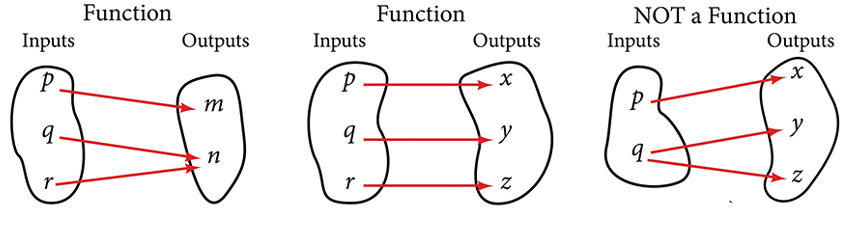
\includegraphics[width = 0.9\textwidth]{img/not-function1.png}}
\end{frame}

\begin{frame}{Functions in Mathematics}

    \begin{center}
        In Mathematics, \textbf{functions are often represented by equations and formulas}    
    \end{center}
    
    \vspace{-0.2cm}
    
    \begin{minipage}{0.5\textwidth}
        
        \begin{block}{\centering Definition of the ``square'' function}
    
            \centering
            \vspace{-0.3cm}
            
            {\Large
            \begin{equation*}
                \tikzmark{name}f(\tikzmark{input}x) = \tikzmark{output}x^2
            \end{equation*}
    
            \begin{tikzpicture}[overlay, remember picture]

                % Name
                \node (name_e) [below of = name, node distance = 0.4cm, anchor = north, xshift = 0.05cm]{\small \textsf{Name}};
            
                \draw[->] (name.south) ++(0.05cm, -0.15cm) to (name_e.north);
    
                % Input
                \node (input_e) [below of = input, node distance = 0.9cm, anchor = north, xshift = 0.3cm] {\small \textsf{Input}};
                
                \draw[->, in = 70, out = 270] (input.south) ++(0.1cm, -0.1cm) to    (input_e.north);
    
                % Output
                \node (output_e) [below of = output, node distance = 0.67cm, xshift = 0.08cm] {\small \textsf{Output}};
        
                \draw[->] (output.south) ++(0.08cm, -0.1cm) to (output_e.north);
    
            \end{tikzpicture}
            } 
        
        % \end{minipage}
        \vspace{0.6cm}
    
        \end{block}
        
    \end{minipage}\hfill
    \begin{minipage}{0.45\textwidth}
        \vspace{0.2cm}
        {\hspace{0.3cm}  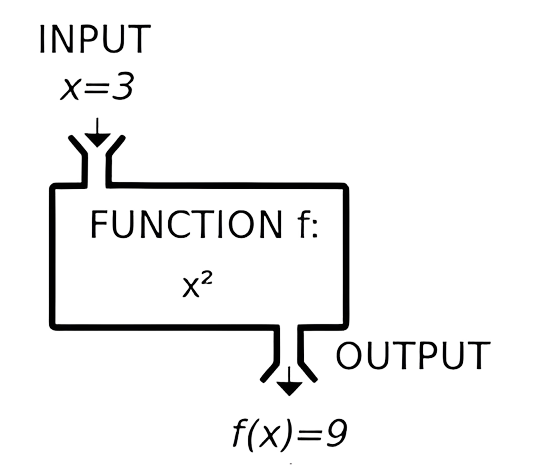
\includegraphics[height = 3.5cm]{img/function2.png}}
    \end{minipage}
    \vspace{0.2cm}

    \begin{block}{Important functions in Mathematics}
         \begin{itemize}[leftmargin = 0.5cm, label = $\bullet$, rightmargin = 0.2cm]
            \item \textbf{Linear function:} $f(x) = ax + b$; \quad
            \textbf{Quadratic function:} $f(x) = ax^2$
            \item \textbf{Cubic function:} $f(x) = ax^3$; \quad 
            \textbf{Polynomial function:} $f(x) = a_0 + a_1x + a_2x^2 + \dots a_nx^n $ %\quad $a_1, \dots, a_n \in \R$, \quad $n\in \N$
            \item \textbf{Exponential function:} $f(x) = e^x$; \quad \textbf{Logarithmic function:} $f(x) = \ln(x)$
            \item \textbf{Trigonometric functions:} $f(x) = \sin(x),\ g(x) = \cos(x) $
        \end{itemize}
    \end{block}

\end{frame}

\begin{frame}{Composition of functions: a function of a function}

    \centering
    Like pipelines, \textbf{we can concatenate functions} to create a ``composite'' function
    
    \begin{minipage}{0.6\textwidth}
        \begin{block}{\centering Creating a composite function}
            Let $f(x) = x^2$, $g(x) = x + 1$, and define
            \begin{align*}
                h(x) &= (g \circ f)(x) = g(f(x)) \\
                     &= g(x^2) = x^2 + 1
            \end{align*}
            \begin{itemize}[leftmargin = 0.5cm, label = $\bullet$, rightmargin = 0.2cm]
                \item \textbf{The domain of $\pmb{g}$ must contain the image of $\pmb{f}$} \\
                That is: $f$'s outputs are $g$'s inputs
                \item \textbf{$\pmb{g\circ f}$ and $\pmb{f\circ g}$ are not necessarily the same} \\
                      ($(f\circ g)(x) = (x + 1)^2 = x^2 + 2x + 1)$)
                \item \textbf{You can compose more than two functions} \\
                      Let $r(x) = x/2$, then $(r\circ g\circ f)(x) = (x^2 + 1)/2$
            \end{itemize}

        \end{block}
    \end{minipage}
    \begin{minipage}{0.35\textwidth}
        \vspace{0.2cm}
        
        {\hspace{0.2cm} 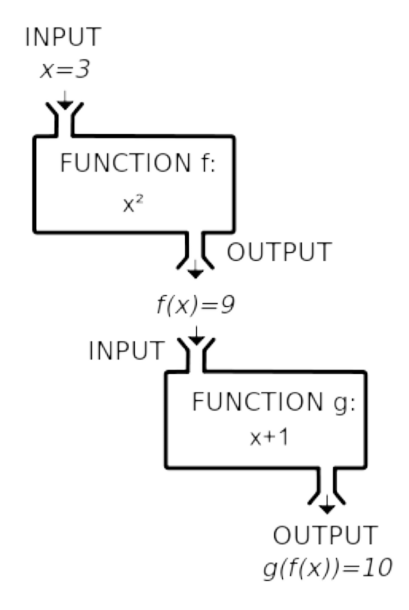
\includegraphics[height = 6cm]{img/function3.png}}
    \end{minipage}
    
\end{frame}

\begin{frame}{Composition of functions - Example}

    \textbf{Problem:} You run an online business that sells sport and nutrition products. To reward your clients you give them two types of discount coupons: the ``save $5\%$ in your next purchase'' (coupon A), and the ``take $5$ dollars off your next purchase'' ones (coupon B). Assuming that you accept both coupons, which one would you apply first? Why?
    \vspace{0.5cm}
    
\end{frame}

\begin{frame}{Composition of functions - Solution}

    \textbf{Solution:} Define the functions $f(x) = 0.95 x$ and $g(x) = x - 5$, with $x \in \R_+$, which represents the price after applying coupons A and B respectively. Define the functions $h(x) = (g\circ f)(x)$ and $r(x) = (f\circ g)(x)$, which are, respectively, the price after applying coupon A first and vice versa. Then,
    \begin{align*}
        h(x) &= g(f(x)) = g(0.95x) = 0.95x - 5 \\
        r(x) &= f(g(x)) = g(x - 5) = 0.95(x - 5) = 0.95x - 4.75
    \end{align*}
    Since $r(x) \geq h(x)$, obtaining the reward associated with $r$ is more convenient, that is, applying coupon $B$ first. \textbf{This strategy yields $\pmb{0.25}$ dollars more.}
        
\end{frame}

\begin{frame}{The inverse function}
    
    Some functions can be ``undone'' to \textbf{find out the input that produced certain output}. 

    \begin{block}{Definition of the inverse of a function}
        \begin{minipage}{0.23\textwidth}
            {\hspace{0.1cm} 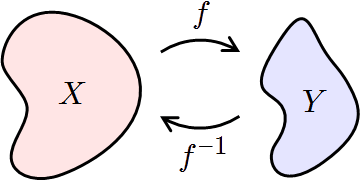
\includegraphics[width = 0.9\textwidth]{img/function-inverse1.png}}
        \end{minipage}
        \begin{minipage}{0.72\textwidth}
            The function $f$ is said to be invertible if, for any $y\in \text{ Img}(f)$ there exists a unique $x\in \text{ Dom}(f)$ such that $f(x) = y$. The inverse of $f$, denoted by $f^{-1}$, is defined as the unique function such that $(f^{-1}\circ f)(x) = x$
        \end{minipage}
    \end{block}    

    \begin{minipage}{0.5\textwidth}
            \begin{block}{Examples}
            \vspace{0.2cm}
            
            \begin{itemize}[leftmargin = 0.5cm, label = $\bullet$, rightmargin = 0.2cm]
                 \item $f(x) = 3x + 8 \Longrightarrow f^{-1}(y) = (y - 8)/3$
                 \item $f(x) = x^2 \Longrightarrow f^{-1}$ does not exist
                 \item $f(x) = x^3 \Longrightarrow f^{-1}(y) = y^{1/3}$
                 \item $f(x) = 1/x \Longrightarrow f^{-1}(y) = 1/y$
            \end{itemize}
        \end{block}
    \end{minipage}
    \begin{minipage}{0.45\textwidth}
        \vspace{0.3cm}
        
        {\hspace{0.3cm} 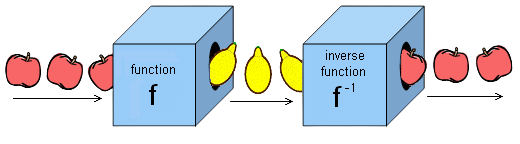
\includegraphics[width = \textwidth, height = 2.3cm]{img/inverse-apple-lemon.png}}
    \end{minipage}
    
    
\end{frame}

\begin{frame}{The graph of a function}

    \textbf{A function can be visually represented} by plotting the set $\{(x, y) : y = f(x)\}$ in the system of coordinates $\R^2$ (or higher dimension if needed)

    \begin{minipage}{0.32\textwidth}
    \centering
    \textbf{Parabolic}
    \vspace{0.3cm}
    
        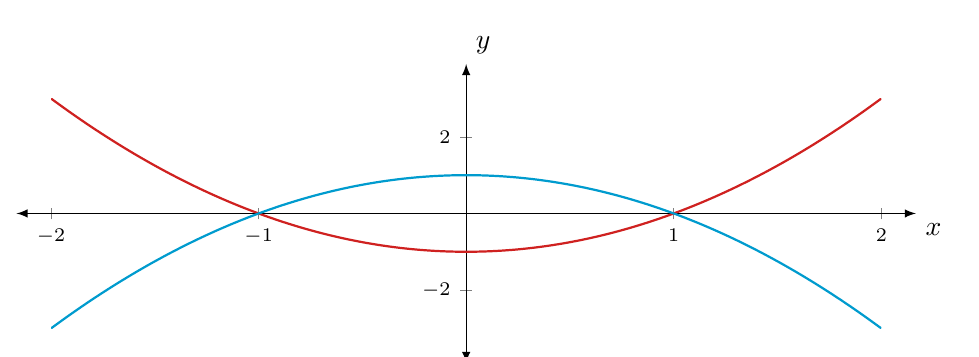
\begin{tikzpicture}
        
        \begin{axis}[
            width=\textwidth,
            height=4.5cm,
            axis lines=middle,
            xmin=-2,
            xmax=2,
            ymin=-3,
            ymax=3,
            xtick={-2, -1, 0, 1, 2},
            % ---------------------------------------------------------------------
            % you don't want the ticks/tick labels to be scaled
            scaled ticks = false,
            %        xticklabels={$20000$},
            % ---------------------------------------------------------------------
            ytick={-4, -2, 2, 4},
            ticklabel style={font=\scriptsize},
            xlabel=$x$,
            ylabel=$y$,
            axis line style={
                latex-latex,
                shorten >=-12.5pt,
                shorten <=-12.5pt,
            },
            xlabel style={at={(ticklabel* cs:1)}, xshift=12.5pt, anchor=north west},
            ylabel style={at={(ticklabel* cs:1)}, yshift=12.5pt, anchor=south west},
        ]

            \addplot[thick, firebrick3, samples = 51, smooth, domain = -2:2] {x^2 - 1};
            \addplot[thick, deepskyblue3, samples = 51, smooth, domain = -2:2] {-x^2 + 1};

        \end{axis}

        \end{tikzpicture}
        \vspace{0.4cm}
        
        $\textcolor{firebrick3}{f(x) = x^2 -1}$ \\
        $\textcolor{deepskyblue3}{f(x) = 1 -  x^2}$
    \end{minipage}
    \begin{minipage}{0.32\textwidth}
    \centering
    \vspace{0.55cm}

    \textbf{Linear}
    \vspace{0.3cm}
    
        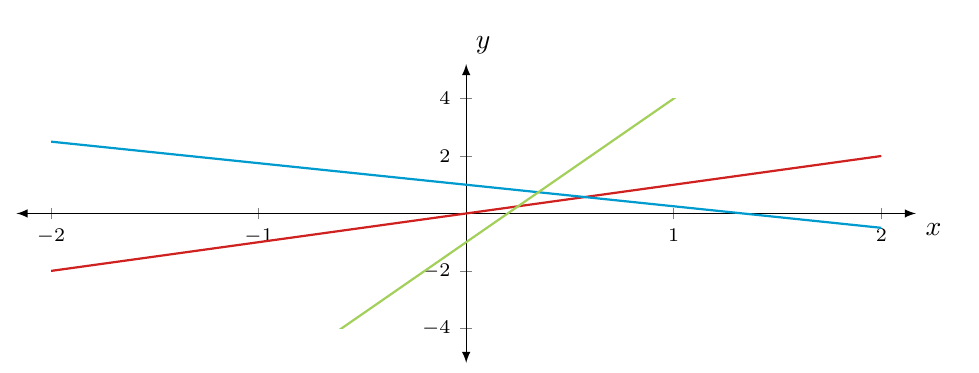
\begin{tikzpicture}
        
        \begin{axis}[
            width=\textwidth,
            height=4.5cm,
            axis lines=middle,
            xmin=-2,
            xmax=2,
            ymin=-4,
            ymax=4,
            xtick={-2, -1, 0, 1, 2},
            % ---------------------------------------------------------------------
            % you don't want the ticks/tick labels to be scaled
            scaled ticks = false,
            %        xticklabels={$20000$},
            % ---------------------------------------------------------------------
            ytick={-4, -2, 2, 4},
            ticklabel style={font=\scriptsize},
            xlabel=$x$,
            ylabel=$y$,
            axis line style={
                latex-latex,
                shorten >=-12.5pt,
                shorten <=-12.5pt,
            },
            xlabel style={at={(ticklabel* cs:1)}, xshift=12.5pt, anchor=north west},
            ylabel style={at={(ticklabel* cs:1)}, yshift=12.5pt, anchor=south west},
        ]

            \addplot[thick, firebrick3, samples = 51, smooth, domain = -2:2] {x};
            \addplot[thick, deepskyblue3, samples = 51, smooth, domain = -2:2] {-0.75*x + 1};
            \addplot[thick, darkolivegreen3, samples = 51, smooth, domain = -2:2] {5*x - 1};
            

        \end{axis}

        \end{tikzpicture}
        \vspace{0.4cm}
        
        $\textcolor{firebrick3}{f(x) = x}$ \\
        $\textcolor{deepskyblue3}{f(x) = -0.75x + 1}$ \\
        $\textcolor{darkolivegreen3}{f(x) = 5x - 1}$
    \end{minipage}
    \begin{minipage}{0.32\textwidth}
    \centering
    \textbf{Exponential / Logarithmic}
    \vspace{0.3cm}
    
        \begin{tikzpicture}
        
        \begin{axis}[
            width=\textwidth,
            height=4.5cm,
            axis lines=middle,
            xmin=-2,
            xmax=2,
            ymin=-4,
            ymax=4,
            xtick={-2, -1, 0, 1, 2},
            % ---------------------------------------------------------------------
            % you don't want the ticks/tick labels to be scaled
            scaled ticks = false,
            %        xticklabels={$20000$},
            % ---------------------------------------------------------------------
            ytick={-4, -2, 2, 4},
            ticklabel style={font=\scriptsize},
            xlabel=$x$,
            ylabel=$y$,
            axis line style={
                latex-latex,
                shorten >=-12.5pt,
                shorten <=-12.5pt,
            },
            xlabel style={at={(ticklabel* cs:1)}, xshift=12.5pt, anchor=north west},
            ylabel style={at={(ticklabel* cs:1)}, yshift=12.5pt, anchor=south west},
        ]

            \addplot[thick, firebrick3, samples = 51, smooth, domain = -2:2] {e^x};
            % \addlegendentry{$x^3$}
            \addplot[thick, deepskyblue3, samples = 51, smooth, domain = 0.005:2] {ln(x)};
            % \addlegendentry{$x^{1/3}$}
            \addplot[dashed, samples = 51, smooth, domain = -2:2] {x};

        \end{axis}

        \end{tikzpicture}
        \vspace{0.4cm}
        
        $\textcolor{firebrick3}{f(x) = e^x}$ \\
        $\textcolor{deepskyblue3}{f^{-1}(x) = \ln(x)}$
    \end{minipage}
     
    
\end{frame}

\begin{frame}{Piecewise-defined function }

    {\hspace{0.3cm}
    \begin{minipage}{0.475\textwidth}
        \centering
        {\hspace{-0.5cm} Absolute value:
        $\textcolor{firebrick3}{f(x) = |x|}$}
        \vspace{0.1cm}
        
        \begin{tikzpicture}
        
        \begin{axis}[
            width=\textwidth,
            height=4.5cm,
            axis lines=middle,
            xmin=-2,
            xmax=2,
            ymin=0,
            ymax=2,
            xtick={-2, -1, 0, 1, 2},
            scaled ticks = false,
            ytick={1, 2, 3},
            ticklabel style={font=\scriptsize},
            xlabel=$x$,
            ylabel=$y$,
            axis line style={
                latex-latex,
                shorten >=-12.5pt,
                shorten <=-12.5pt,
            },
            xlabel style={at={(ticklabel* cs:1)}, xshift=12.5pt, anchor=north west},
            ylabel style={at={(ticklabel* cs:1)}, yshift=12.5pt, anchor=south west},
        ]

            \addplot[thick, firebrick3, samples = 51, smooth, domain = -2:0] {-x};
            \addplot[thick, firebrick3, samples = 51, smooth, domain = 0:2] {x};
            

        \end{axis}

        \end{tikzpicture}
                
    \end{minipage}
    \begin{minipage}{0.475\textwidth}
        \centering
        {\hspace{-0.4cm} Indicator: 
        $\textcolor{deepskyblue3}{f(x) = \Ind_{(0, \infty)}(x) + 0.5}$}
        \vspace{0.1cm}
        
        \begin{tikzpicture}
        
        \begin{axis}[
            width=\textwidth,
            height=4.5cm,
            axis lines=middle,
            xmin=-2,
            xmax=2,
            ymin=0,
            ymax=2,
            xtick={-2, -1, 0, 1, 2},
            scaled ticks = false,
            ytick={1, 2, 3},
            ticklabel style={font=\scriptsize},
            xlabel=$x$,
            ylabel=$y$,
            axis line style={
                latex-latex,
                shorten >=-12.5pt,
                shorten <=-12.5pt,
            },
            xlabel style={at={(ticklabel* cs:1)}, xshift=12.5pt, anchor=north west},
            ylabel style={at={(ticklabel* cs:1)}, yshift=12.5pt, anchor=south west},
        ]

            \addplot[thick, deepskyblue3, samples = 51, smooth, domain = -2:0] {1.5};
            \addplot[thick, deepskyblue3, samples = 51, smooth, domain = 0:2] {0.5};

            \addplot[deepskyblue3, mark = ] coordinates {(0, 0.5)} node[] {$\bullet$};
            \addplot[deepskyblue3, mark = ] coordinates {(0, 1.5)} node[] {$\pmb{\circ}$};
            
        \end{axis}

        \end{tikzpicture}
            
    \end{minipage}
    }
    \vspace{0cm}

    \begin{minipage}{0.3\textwidth}
        \begin{align*}
        \color{firebrick3}
        |x| & \color{firebrick3}= 
        \begin{cases}
            -x & \text{if } x \leq 0 \\
            x & \text{if } x > 0
        \end{cases} \\
        \color{deepskyblue3} 
        \Ind_{(0,\infty)}(x) & \color{deepskyblue3}= 
        \begin{cases}
            0 & \text{if } x \leq 0 \\
            1 & \text{if } x > 0
        \end{cases}
        \end{align*} 
    \end{minipage}
    \begin{minipage}{0.4\textwidth}
        \begin{align*}
        f (x) = 
        \begin{cases}
            g_1(x) & \text{if } x\in A_1 \\
            g_2(x) & \text{if } x\in A_2 \\
            \quad \vdots & \quad\ \ \vdots \\
            g_2(x) & \text{otherwise}
        \end{cases}
        \end{align*}
    \end{minipage}
    \begin{minipage}{0.25\textwidth}
        \vspace{0.25cm}
        
        A \textbf{piecewise function} is defined by multiple \textbf{sub-functions}, each applied to a different \textbf{subset of the domain}
    \end{minipage}
    
    
\end{frame}

\begin{frame}{Functions of two variables}

    Sometimes it is useful to study \textbf{functions whose domain is a subset of} $\pmb{R^2}$. Graphically, they are represented by a \textbf{surface} in a $\pmb{3}$\textbf{-dimensional coordinate system} 
    \vspace{0.2cm}

    \begin{minipage}{0.5\textwidth}
        
        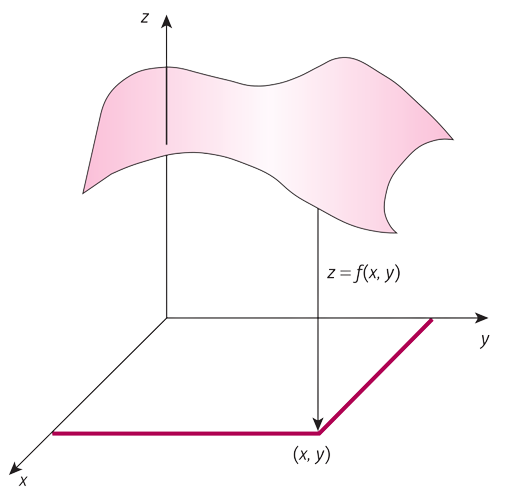
\includegraphics[width = 0.95\textwidth, height = 4.8cm]{img/2-variables.png}    
    \end{minipage}\hspace{0.4cm}
    \begin{minipage}{0.45\textwidth}
    \begin{block}{Examples}
        \vspace{0.1cm}
        
        \begin{itemize}[leftmargin = 0.5cm, label = $\bullet$, rightmargin = 0.2cm]
                 \item \textbf{Topography:} \\ $f($Latitude, Altitude$) =$ Height
                 \item \textbf{Production:} \\ $f($Capital, Labour$) =$ Output
                 \item \textbf{Investment value:} \\ $f($Time, Return rate$) =$ Value
                 \item \textbf{Consumer Behavior:} \\ $f($Price, Income$) =$ Consumption
        \end{itemize}         
    \end{block}
    \end{minipage}
    
\end{frame}

\begin{frame}{Functions of more than two variables}

    Functions of many variables extend the concept of functions from two variables to any number of variables. 
    
    \begin{block}{Examples of functions of many variables}
        \begin{itemize}[leftmargin = 0.5cm, label = $\bullet$, rightmargin = 0.2cm]
            \item \textbf{Meteorology:} \\ $f($x, y, z, t$) =$ Temperature variations in the atmosphere at different altitudes ($z$), geographic positions ($x, y$), and time ($t$).
            \item \textbf{Geology: Seismic Activity} \\ $f($x, y, z, t$) =$ Magnitude of an earthquake at an specific geographic location $(x, y, z)$ and time $t$
            \item \textbf{Economics: Utility Function} \\
            $f(x_1, x_2, \dots, x_n) =$ Individuals' utility based on their consumption of multiple goods %$(x_1, x_2, \dots, x_n)$
        \end{itemize}   
    \end{block}
      
\end{frame}
%----------------------- FUNCTIONS -----------------------%

%----------------------- ECONOMIC APPLICATION -----------------------%
\section{Economical application: 
         Supply and Demand in a single-good market}

\begin{frame}{Supply and Demand}

    \textbf{Supply and Demand sets}
    \begin{itemize}[leftmargin = 0.5cm, label = $\bullet$, rightmargin = 0.2cm]
        \item $S = \{(q, p)\ |\ \text{ if $p$ was the selling price, $q$ would be the amount supplied}\}$
        \item $D = \{(q, p)\ |\ \text{ if $p$ was the selling price, $q$ would be the quantity sold (demand)}\}$
    \end{itemize}

    \begin{block}{Supply-Demand equilibrium}
        \textbf{Problem:} Suppose we know all about the factors affecting supply and demand in the market for a particular good; in other words, the \textbf{supply set} $S$ and the \textbf{demand set} $D$ are given. What values of $q$ and $p$ will actually be achieved in the market?

        \textbf{Solution:} The solution is to find the intersection of $D$ and $S$, called the \textbf{equilibrium set} $E$, because that is where the quantity supplied is exactly balanced by the quantity required.
        \textbf{How to find the $\pmb{E = S\cap D}$?}
    \end{block}
    
\end{frame}

\begin{frame}{Supply-Demand equilibrium}

    When \textbf{the supply and demand sets are plotted} in the Cartesian coordinate system, they usually exhibit a \textbf{functional representation} with a smooth increasing (law of supply) and decreasing (law of demand) behavior, respectively
    \vspace{0.2cm}
    
    \begin{minipage}{0.4\textwidth}
    \centering
    % \vspace{0.55cm}
    {\hspace{0.5cm}
        \begin{tikzpicture}
        
        \begin{axis}[
            width=\textwidth,
            height=5cm,
            axis lines=middle,
            xmin=0,
            xmax=2,
            ymin=0,
            ymax=5,
            xtick={\empty},
            % ---------------------------------------------------------------------
            % you don't want the ticks/tick labels to be scaled
            scaled ticks = false,
            %        xticklabels={$20000$},
            % ---------------------------------------------------------------------
            ytick={\empty},
            ticklabel style={font=\scriptsize},
            xlabel=$q$,
            ylabel=$p$,
            axis line style={
                latex-latex,
                shorten >=-12.5pt,
                shorten <=-12.5pt,
            },
            xlabel style={at={(ticklabel* cs:1)}, xshift=12.5pt, anchor=north west},
            ylabel style={at={(ticklabel* cs:1)}, yshift=12.5pt, anchor=south west},
        ]

            % \coordinate (P) at (1.1814, 1.5387);
             
            \addplot[thick, firebrick3, samples = 51, smooth, domain = 0.2:2] {x^1.75 + 0.6};
            \addplot[thick, deepskyblue3, samples = 51, smooth, domain = 0.2:2] {(x - 2.5)^2 + 0.2};

            \addplot[mark = *] coordinates {(1.1814, 1.95)} node[] {};
            \addplot[mark = ] coordinates {(1.155, 1.3)} node[] {$E$};

            \addplot[] coordinates {(1.7, 2.5)} node[] {$\textcolor{firebrick3}{q_S}$}; 
            \addplot[] coordinates {(0.4, 3.8)} node[] {$\textcolor{deepskyblue3}{q_D}$};

        \end{axis}

        \end{tikzpicture}
        }
    \end{minipage}\hspace{0.4cm}
    \begin{minipage}{0.55\textwidth}
        \begin{itemize}[leftmargin = 0.3cm, label = $\bullet$, rightmargin = 0cm]
            \item The supply and demand sets (often) admit a functional representation: \\
                  $\textcolor{firebrick3}{S = \{(q, p)\ |\ q = q_S(p)\}}$, \quad $\textcolor{deepskyblue3}{D = \{(q, p)\ |\ q = q_D(p)\}}$ 
            \item $\textcolor{firebrick3}{q_S}$: \textbf{supply function}, \quad $\textcolor{deepskyblue3}{q_D}$: \textbf{demand function}
            \item We can also express $p$ in terms of $q$: \\
                  $\textcolor{firebrick3}{S = \{(q, p)\ |\ p = p_S(q)\}}$, \quad $\textcolor{deepskyblue3}{D = \{(q, p)\ |\ p = p_D(q)\}}$
            \item $\textcolor{firebrick3}{p_S}$: \textbf{inverse supply function} \\
                  $\textcolor{deepskyblue3}{p_D}$: \textbf{inverse demand function}
        \end{itemize}
        
    \end{minipage}
    
\end{frame}

\begin{frame}{Example of supply-demand equilibrium. Problem}

    \begin{block}{Supply-demand equilibrium in the catfood market}
        
        \begin{minipage}{0.35\textwidth}
            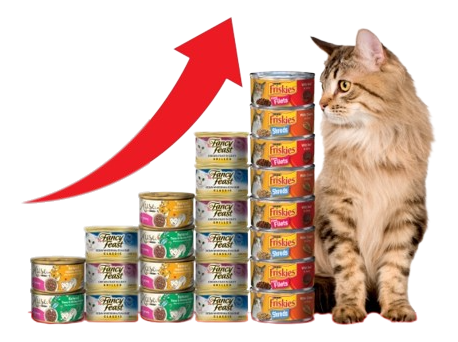
\includegraphics[width = 0.9\textwidth]{img/catfood.png}
        \end{minipage}
        \begin{minipage}{0.6\textwidth}
            Assume that the catfood market is described by the supply and demand sets 
            \begin{align*}
                \textcolor{firebrick3}{S} &\textcolor{firebrick3}{= \{(q,p)\ |\ 5p- q^2 -2q = 27\}} \\
                \textcolor{deepskyblue3}{D} &\textcolor{deepskyblue3}{= \{(q,p)\ |\ p + q^2 +2q = 15\}}
            \end{align*}
            Write down $p_S$ and $p_D$, sketch $S$ and $D$. \\
            Determine the equilibrium set $E = S \cap D$ and comment on the economical equilibrium.
        \end{minipage}
    \end{block}
    
\end{frame}

\begin{frame}{Example of supply-demand equilibrium. Solution}
    
    \begin{minipage}{0.4\textwidth}
    \centering
    \vspace{0.3cm}
    
    {\hspace{0.6cm}
        \begin{tikzpicture}
        
        \begin{axis}[
            width=\textwidth,
            height=5.8cm,
            axis lines=middle,
            xmin=0,
            xmax=3,
            ymin=0,
            ymax=15,
            xtick={\empty},
            % ---------------------------------------------------------------------
            % you don't want the ticks/tick labels to be scaled
            scaled ticks = false,
            %        xticklabels={$20000$},
            % ---------------------------------------------------------------------
            ytick={\empty},
            ticklabel style={font=\scriptsize},
            xlabel=$q$,
            ylabel=$p$,
            axis line style={
                latex-latex,
                shorten >=-12.5pt,
                shorten <=-12.5pt,
            },
            xlabel style={at={(ticklabel* cs:1)}, xshift=12.5pt, anchor=north west},
            ylabel style={at={(ticklabel* cs:1)}, yshift=12.5pt, anchor=south west},
        ]

            % \coordinate (P) at (1.1814, 1.5387);
             
            \addplot[thick, firebrick3, samples = 51, smooth, domain = 0:3] {(27 + 2*x + x^2)/5};
            \addplot[thick, deepskyblue3, samples = 51, smooth, domain = 0:3] {15 - x^2 - 2*x};

            \addplot[mark = *] coordinates {(2, 7)} node[] {};
            \addplot[mark = ] coordinates {(1.96, 5.8)} node[] {$E$};

            \addplot[] coordinates {(0.8, 4.5)} node[] {$\textcolor{firebrick3}{q_S}$}; 
            \addplot[] coordinates {(0.8, 11)} node[] {$\textcolor{deepskyblue3}{q_D}$};

        \end{axis}

        \end{tikzpicture}
        }
    \end{minipage}\hspace{0.4cm}
    \begin{minipage}{0.55\textwidth}
        \begin{itemize}[leftmargin = 0.3cm, label = $\bullet$, rightmargin = 0cm]
            \item  \textbf{Supply and demand functions:} \\
            $\textcolor{firebrick3}{p_S(q) = (q^2 + 2q + 27)/5}$ \\
            $\textcolor{deepskyblue3}{p_D(q) = 15 - q^2 - 2q}$

            \item \textbf{Equilibrium set:} Solve the equation 
            \vspace{-0.1cm}
            \begin{align*}
                                    && p_D(q) &= p_S(q) \\
                \Longleftrightarrow && 15 - q^2 - 2q &= (q^2 + 2q + 27)/5 \\
                \stackrel{*5}{\Longleftrightarrow} && 6q^2 + 12q - 48 &= 0 \\
                \stackrel{/6}{\Longleftrightarrow} && q^2 + 2q - 8 &= 0 \\
                \Longleftrightarrow && (q + 4)(q - 2) &= 0
            \end{align*}
            Therefore, $E = \{(-4, 7), (2, 7)\}$.
        \end{itemize}
        
    \end{minipage}
    \vspace{-0.2cm}
    
    \begin{itemize}[leftmargin = 0.3cm, label = $\bullet$, rightmargin = 0cm]
        \item \textbf{Economic equilibrium:} \\
              The point $(-4, 7$) has no economic significance because $q$ represents a quantity of a real commodity, so $q = -4$ is meaningless. The economic equilibrium is therefore given by $q^* = 2$ and $p^* = 7$.
    \end{itemize}
    
\end{frame}

\begin{frame}{A short note on factorization. General rule}

\begin{block}{General rule (product–sum form)}
\begin{minipage}{0.65\textwidth}
    
    For \(a,b,c,d \in \R\),
    \[
      (cx+a)(dx+b)=cd\,x^{2}+(ad+bc)x+ab.
    \]
    To factor \(Ax^{2}+Bx+C\), find \(c,d,a,b\) such that
    \[
      cd=A,\qquad ab=C,\qquad ad+bc=B.
    \]
\end{minipage}
\begin{minipage}{0.3\textwidth}

    \begin{center}
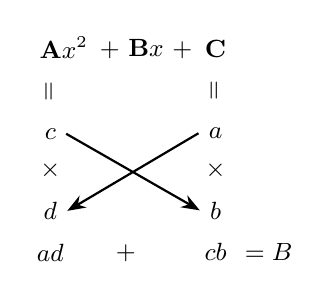
\begin{tikzpicture}[
  >=Stealth, thick,
  every node/.style={font=\small}
]
  % Top labels
  \node (At) {$\mathbf{A}x^2$};
  \node (Bt) [right=-1.1mm of At,yshift=-0.2mm] {$+\ \mathbf{B}x\ +$};
  \node (Ct) [right=-1mm of Bt] {$\mathbf{C}$};

  % Factors under A and C
  \node (eqA) [below=0.3mm of At,xshift=-1.7mm] {$\verteq$};
  \node (c) [below=0.3mm of eqA] {$c$};
  \node (plusA) [below=0.3mm of c] {$\times$};
  \node (d) [below=0.3mm of plusA] {$d$};
  \node (ad) [below=0.5mm of d] {$ad$};
  \node (cross_plus) [right=4mm of ad] {$+$};

  \node (eqC) [below=0.3mm of Ct] {$\verteq$};
  \node (a) [below=0.3mm of eqC] {$a$};
  \node (plusC) [below=0.3mm of a] {$\times$};
  \node (b) [below=0.3mm of plusC] {$b$};
  \node (cb) [below=0.5mm of b] {$cb$};
  \node (eqB) [right=-0.3mm of cb] {$= B$};
  

  % Cross arrows and products
  \draw[->] (c.east) -- (b.west) node[midway, above, sloped] {};
  \draw[<-] (d.east) -- (a.west) node[midway, below, sloped] {};
\end{tikzpicture}
\end{center}
\end{minipage}
\end{block}
\vspace{0.2cm}

\begin{minipage}{0.65\textwidth}
  \textbf{Example:} factor \(6x^{2}+11x+3\)
    \begin{itemize}[label=$\bullet$]
      \item Identify \(A=6,\;B=11,\;C=3\).
      \item Try factors: \(cd=6\Rightarrow(3,2)\); \(ab=3\Rightarrow(1,3)\).
      \item Check the middle term: \(ad+bc=11=B\).
      \item Therefore \(6x^{2}+11x+3=(3x+1)(2x+3)\).
    \end{itemize}
    % \vspace{2pt}
    % \emph{Sign tip:} if \(C<0\), choose \(a,b\) with opposite signs so \(ab=C\), then pick signs so \(ad+bc=B\).
\end{minipage}
\begin{minipage}{0.3\textwidth}
    \begin{center}
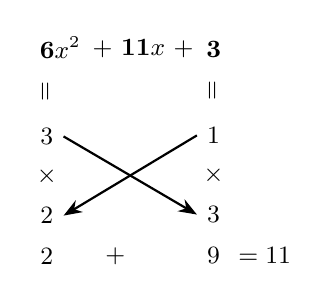
\begin{tikzpicture}[
  >=Stealth, thick,
  every node/.style={font=\small}
]
  % Top labels
  \node (At) {$\mathbf{6}x^2$};
  \node (Bt) [right=-1.1mm of At,yshift=-0.2mm] {$+\ \mathbf{11}x\ +$};
  \node (Ct) [right=-1mm of Bt] {$\mathbf{3}$};

  % Factors under A and C
  \node (eqA) [below=0.3mm of At,xshift=-1.7mm] {$\verteq$};
  \node (c) [below=0.3mm of eqA] {$3$};
  \node (plusA) [below=0.3mm of c] {$\times$};
  \node (d) [below=0.3mm of plusA] {$2$};
  \node (ad) [below=0.5mm of d] {$2$};
  \node (cross_plus) [right=4mm of ad] {$+$};

  \node (eqC) [below=0.3mm of Ct] {$\verteq$};
  \node (a) [below=0.3mm of eqC] {$1$};
  \node (plusC) [below=0.3mm of a] {$\times$};
  \node (b) [below=0.3mm of plusC] {$3$};
  \node (cb) [below=0.5mm of b] {$9$};
  \node (eqB) [right=-0.3mm of cb] {$= 11$};
  

  % Cross arrows and products
  \draw[->] (c.east) -- (b.west) node[midway, above, sloped] {};
  \draw[<-] (d.east) -- (a.west) node[midway, below, sloped] {};
\end{tikzpicture}
\end{center}
\end{minipage}
\end{frame}

% \begin{frame}{A short note on factorization}

%   % Put this inside a frame or anywhere you want the figure



% \end{frame}

\begin{frame}{A short note on factorization. Special-case rules and Discriminant}

    \begin{block}{Factorization rules}
        All of these special-case rules follow from the general rule
        \begin{itemize}[leftmargin = 0.5cm, label = $\bullet$ , rightmargin = 0.2cm]
            % \item \textbf{Rule 1}\quad $cdx^2 + (ad + bc)x + ab = (cx + a)(dx + b)$
            \item $x^2 + (a + b)x + ab = (x + a)(x + b)$
            \item $x^2 + 2ax + a^2 = (x + a)^2 $
            \item $x^2 - 2ax + a^2 = (x - a)^2$
            \item $x^2 - a^2 = (x + a)(x - a)$
        \end{itemize}

    \end{block}
    \vspace{0.5cm}
    
    \begin{block}{Discriminant rule}
        For the quadratic polynomial $f(x) = ax^2 + bx + c$, $D = b^2 - 4ac$ is the discriminant

        \begin{itemize}[leftmargin = 0.5cm, label = $\bullet$, rightmargin = 0.2cm]
            \item if $D < 0$, the polynomial cannot be factorized using real coefficients
            \item if $D = 0$, $f(x) = (x + b/2a)^2$
            \item if $D > 0$, $f(x) = (x - (-b + \sqrt{D})/2a)((x - (-b - \sqrt{D})/2a))$
        \end{itemize}
        
    \end{block}
    
\end{frame}
%----------------------- ECONOMIC APPLICATION -----------------------%

%----------------------- SEQUENCE AND LIMITS -----------------------%
\section{Sequences and limits}

\begin{frame}{Sequences}

    \begin{block}{Definition of a sequence}
        A sequence (or progression) is a list of numbers (or objects) arranged in a specific order, following a pattern
    \end{block}

    \begin{itemize}[leftmargin = 0.5cm, label = $\bullet$, rightmargin = 0.2cm]
        \item \textbf{Notation:} Subscripts are often used. $(x_0, x_1, x_2, \dots)$ or $x_n$, $n\in \N$ 
        \item \textbf{Interpretation:} Represents the evolution of a quantity over time
        \item \textbf{Recurrence equation:} Relates $x_n$ in terms of $x_{n - 1}, \dots, x_1$. Also known as \textbf{difference equation}
        \item \textbf{Solution:} Relates $x_n$ in terms of $n$
    \end{itemize}
    % \vspace{0.3cm}
    

    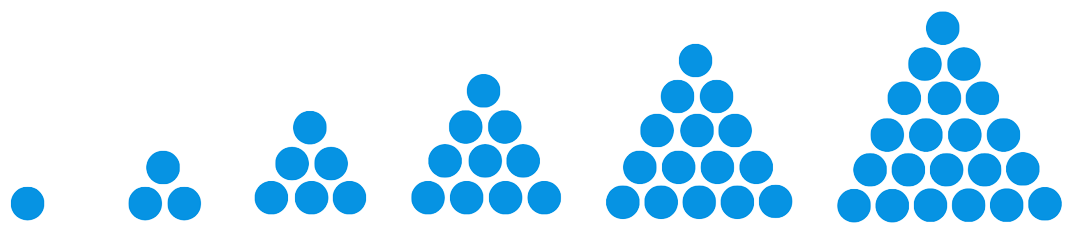
\includegraphics[width = \textwidth]{img/sequence.png}
    
    
    
\end{frame}

\begin{frame}{Example of recurrent sequences}

    \begin{minipage}{0.3\textwidth}
        {\hspace{0.1cm} 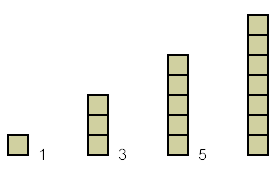
\includegraphics[width = 0.91\textwidth]{img/arithmetic-2.png}}
        \vspace{0.25cm}
        
    \end{minipage}
    \begin{minipage}{0.65\textwidth}
        \begin{itemize}[leftmargin = 0.5cm, label = $\bullet$, rightmargin = -0.2cm]
            \item \textbf{Arithmetic:} $x_n = x_{n-1} + a$, $a \in\R$. $3, 5, 7, 9, 11, \dots$\\
            \textbf{Example:} Loan payments, salary increases based on fixed amounts 
        \end{itemize}
    
    \end{minipage}
    \vspace{0.3cm}

    \begin{minipage}{0.3\textwidth}
        
        {\hspace{0.1cm} 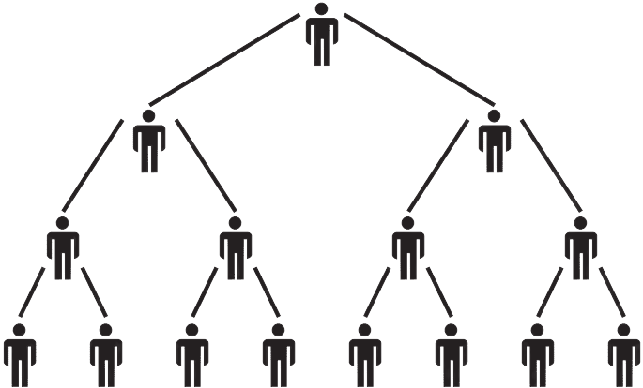
\includegraphics[width = 0.91\textwidth]{img/geometric.png}}
        \vspace{0.4cm}
        
    \end{minipage}
    \begin{minipage}{0.65\textwidth}
        \begin{itemize}[leftmargin = 0.5cm, label = $\bullet$, rightmargin = -0.2cm]
        
        \item \textbf{Geometric:} $x_n = ax_{n-1}$, $a \in R$. $2, 4, 8, 16, 32, \dots$ \\
        \textbf{Example:} Cell Division, compound interest          
    \end{itemize}
    
    \end{minipage}
    
\end{frame}

\begin{frame}{Solution of a sequence}

    We say that $f(n)$ is \textbf{the solution of the sequence} $x_n$, $n\in\N$, if $x_n = f(n)$. That is, the $n^{\text{th}}$ term is expressed in terms of the time $n$ and not via the recurrence equation

    \begin{block}{Solution of a linear first-order recurrence sequence}
        \textbf{Recurrence equation:} $x_n = a x_{n-1} + b$,\quad $a, b \in \R$, $a\neq 1$ \\
        \vspace{0.2cm}
        
        \textbf{Solution:}
        \vspace{-0.2cm}
        
        \begin{itemize}[leftmargin = 0.5cm, label = $\bullet$, rightmargin = 0.2cm]
            \item Find the \textbf{time-independent solution}: $x^* = a x^* + b \Rightarrow x^* = b/(1-a)$
            \item Find the (time-dependent) solution of $y_n = x_n - x^*$:
            \begin{align*}
                y_n + x^* = a(y_{n-1} + x^*) + b \Longleftrightarrow y_n = ay_{n-1} \Longleftrightarrow y_n = a^n y_0
            \end{align*}
            \item Recover the (time-dependent) solution of $x_n$:
            $$
            x_n = y_n + x^* = a^ny_0 + x^* = a^n(x_0 - x^*) + x^*
            $$
        \end{itemize}
    \end{block}
    
\end{frame}

\begin{frame}{Limit of a sequence}

    \begin{minipage}{0.4\textwidth}
        {\hspace{0.1cm}
        \begin{tikzpicture}
        
        \begin{axis}[
            width = 0.93\textwidth,
            height = 3cm,
            axis lines = middle,
            xmin = 0,
            xmax = 10.25,
            ymin = 0,
            ymax = 1.1,
            xtick = {1, 2, 10},
            scaled ticks = false,
            ytick={1, 1/2, 1/10},
            ticklabel style = {font=\scriptsize},
            xlabel=$n$,
            ylabel=$x_n$,
            axis line style={
                -latex,
                shorten >= -0.3cm,
                % shorten <=-12.5pt,
            },
            xlabel style={at={(ticklabel* cs:1)}, xshift = 0.2cm, anchor=north west},
            ylabel style={at={(ticklabel* cs:1)}, yshift = 0.2cm, anchor=south west},
        ]

            \addplot[mark = ] coordinates {(1, 1)} node[] {$\boldsymbol{\cdot}$};
            \addplot[mark = ] coordinates {(2, 1/2)} node[] {$\boldsymbol{\cdot}$};
            \addplot[mark = ] coordinates {(3, 1/3)} node[] {$\boldsymbol{\cdot}$};
            \addplot[mark = ] coordinates {(4, 1/4)} node[] {$\boldsymbol{\cdot}$};
            \addplot[mark = ] coordinates {(5, 1/5)} node[] {$\boldsymbol{\cdot}$};
            \addplot[mark = ] coordinates {(6, 1/6)} node[] {$\boldsymbol{\cdot}$};
            \addplot[mark = ] coordinates {(7, 1/7)} node[] {$\boldsymbol{\cdot}$};
            \addplot[mark = ] coordinates {(8, 1/8)} node[] {$\boldsymbol{\cdot}$};
            \addplot[mark = ] coordinates {(9, 1/9)} node[] {$\boldsymbol{\cdot}$};
            \addplot[mark = ] coordinates {(10, 1/10)} node[] {$\boldsymbol{\cdot}$};

        \end{axis}

        \end{tikzpicture}
        }
    \end{minipage}
    \begin{minipage}{0.55\textwidth}
        Consider the \textit{(harmonic) sequence} $x_n = 1/n$ \\

        $1, 1/2, 1/3, 1/4, \dots, 1/10, \dots, 1/100, \dots$ \\

        \textbf{What number is the sequence approaching?}
    \end{minipage}
    \vspace{0.1cm}
    
    \begin{block}{Definition of the limit of a sequence (Informal)}
        The limit of a sequence, if it exists, is the value their terms approach as the index goes to infinity
    \end{block}

    \textbf{Limits are essentials} for advanced mathematics. They underpin derivatives, integrals, and the fundamental concepts of calculus

\end{frame}

\begin{frame}{Convergence, divergence, and non-existing limits}

    \begin{itemize}[leftmargin = 0.5cm, label = $\bullet$, rightmargin = 0.2cm]
    
        \item Some sequences approach a (finite) value as their terms' indexes go to infinite. Those are called \textbf{convergent sequences}, and the approached value is the limit \\

        \textbf{Example:}\ $x_n = 1/n$, \quad $x_n = 2^{-n}$ \\
        \vspace{0.2cm}

        \item Other sequences grow or decay indefinitely, surpassing any number, as large as it might be. Those are called \textbf{divergent sequences}. In such a case it is said that the limit is infinite \\

        \textbf{Example:}\ $x_n = -n$, \quad $x_n = 2^n$ \\
        \vspace{0.2cm}

        \item The remaining sequences, those that neither converge nor diverge, are said to have no limit \\

        \textbf{Example:}\ $x_n = (-1)^n$

    \end{itemize}

\end{frame}

\section{\mbox{Economical application: the cobweb model}}

\begin{frame}{Economical application: the cobweb model}

    \begin{itemize}[leftmargin = 0.5cm, label = $\bullet$, rightmargin = 0.2cm]
        \item[1.] \textbf{Scenario:} Corn Market Fluctuation

        \item[2.] \textbf{Year 0 - Shortage and Price Increase:} 
        A severe drought causes a \textbf{drop in corn production}, which results in a shortage and leads to an \textbf{increase in corn prices}. These initial diminished quantity and increased price are denoted by $q_0$ and $p_0 = p_D(q_0)$
    
        \item[3.] \textbf{Year 1 - Increased Quantity:} 
        Farmers, anticipating continued high prices as in Year 0, \textbf{increase their corn production}, causing a surplus in the market and, consequently, a \textbf{drop in corn prices}. These increased quantity and plumed price are denoted by $q_1 = q_S(p_0)$, $p_1 = p_D(q_1)$

        \item[4.] \textbf{Cycle:}
        The cycle goes on between shortage, price increase, increased production, and dropped prices. Two sequences are created with the initial condition $q_0$ and the dynamics
        $$
        q_n = q_S(p_{n-1}), \quad p_n = p_D(q_n)
        $$
    \end{itemize}

\end{frame}

\begin{frame}{An example of the cobweb model}

    \begin{block}{Problem}
        Let the corn market described in the previous slide has supply and demand sets
        $$
        D = \{(q, p)\ |\ q + p = 24\},\quad S = \{(q, p)\ |\ 2q + 18 = p\}
        $$
        Obtain the prices $p_n$ for an initial shrinkage $q_0 = 0.5$. Proof that $p^* = \lim_{n\rightarrow\infty}p_n$     
    \end{block}

    \begin{block}{Solution}
        
        \begin{minipage}{0.5\textwidth}
            {\hspace{0.1cm}
        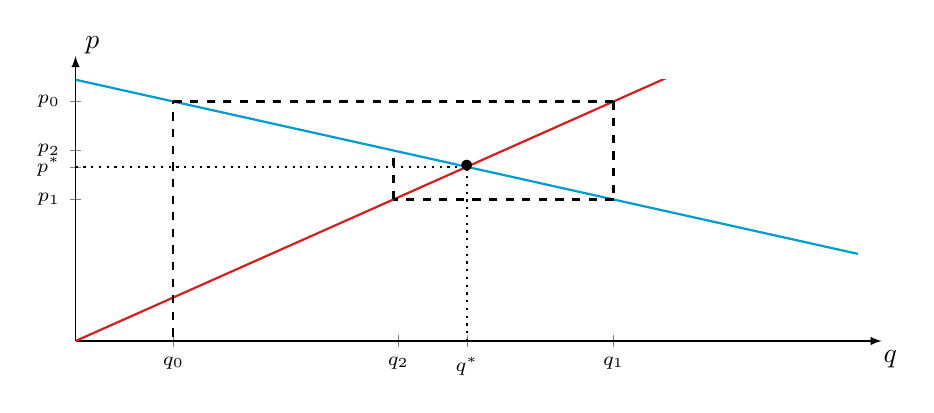
\begin{tikzpicture}
        
        \begin{axis}[
            width = 0.95\textwidth,
            height = 4.9cm,
            axis lines = middle,
            xmin = 0,
            xmax = 4,
            ymin = 18,
            ymax = 24,
            xtick = {0.5, 1.65, 2, 2.75},
            xticklabels = {$q_0$, $q_2$, $q^*$, $q_1$},
            scaled ticks = false,
            ytick = {21.25, 22, 22.375, 23.5},
            yticklabels = {$p_1$, $p^*$, $p_2$, $p_0$},
            ticklabel style = {font=\scriptsize},
            xlabel = $q$,
            ylabel = $p$,
            axis line style = {
                -latex,
                shorten >= -0.3cm,
                % shorten <=-12.5pt,
            },
            xlabel style={at={(ticklabel* cs:1)}, xshift = 0.2cm, anchor=north west},
            ylabel style={at={(ticklabel* cs:1)}, yshift = 0.2cm, anchor=south west},
        ]

            \addplot[thick, firebrick3, samples = 51, smooth, domain = 0:4] {2*x + 18};
            \addplot[thick, deepskyblue3, samples = 51, smooth, domain = 0:4] {24 - x};

            \addplot[mark = ] coordinates {(2, 22)} node[] {$\bullet$};
            % \addplot[mark = ] coordinates {(1.96, 20)} node[] {$E$};

            % cobweb
            \draw[dashed, thick] (axis cs:0.5, 18.1) -- (axis cs:0.5, 23.5);
            \draw[dashed, thick] (axis cs:0.5, 23.5) -- (axis cs:2.75, 23.5);
            \draw[dashed, thick] (axis cs:2.75, 23.5) -- (axis cs:2.75, 21.25);
            \draw[dashed, thick] (axis cs:2.75, 21.25) -- (axis cs:1.625, 21.25);
            \draw[dashed, thick] (axis cs:1.625, 21.25) -- (axis cs:1.625, 22.375);

            % dotted lines
            \draw[dotted, thick] (axis cs:2, 18) -- (axis cs:2, 22);
            \draw[dotted, thick] (axis cs:0, 22) -- (axis cs:2, 22);

        \end{axis}

        \end{tikzpicture}
        }    
        \end{minipage}
        \begin{minipage}{0.45\textwidth}
        \vspace{-0.4cm}
        
            \begin{align*}
                                &\;\; q_S(p) = 0.5p - 9, \quad p_D(q) = 24 - q \\
                \Longrightarrow &\;\; q_n = 0.5p_{n-1} - 9, \quad p_n = 24 - q_n \\
                \Longrightarrow &\;\; p_n = 33 - 0.5p_{n-1} \\
                \Longrightarrow &\;\; p_n = 22 + (p_0 - 22)(-0.5)^n \\
                \Longrightarrow &\;\; \lim_{n} p_n = 22 = p^* \\
                                &\;\; q_0 = 0.5,\quad p_0 = 23.5, \\ 
                                &\;\; q_1 = 2.75,\quad p_1 = 21.25, \\
                                &\;\; q_2 = 1.625,\quad p_2 = 22.375, \dots  
            \end{align*}     
        \end{minipage}
        
    \end{block}

\end{frame}

\end{document}
